\documentclass[openany,oneside]{book}

\usepackage{amsmath, amsthm, amssymb, amsfonts}
\usepackage{mathtools}
\usepackage{booktabs}
\usepackage{thmtools}
\usepackage{graphicx}
\usepackage{setspace}
\usepackage{geometry}
\usepackage{float}
\usepackage{hyperref}
\usepackage[utf8]{inputenc}
\usepackage[english]{babel}
\usepackage{framed}
\usepackage[dvipsnames]{xcolor}
\usepackage{tcolorbox}
\usepackage{bm}
\usepackage{float}
\usepackage{physics}
\usepackage{enumitem}
\usepackage{cancel}
\usepackage{titlesec}

\colorlet{LightGray}{White!90!Periwinkle}
\colorlet{LightOrange}{Orange!15}
\colorlet{LightGreen}{Green!15}

\newcommand{\HRule}[1]{\rule{\linewidth}{#1}}

\declaretheoremstyle[name=Theorem,]{thmsty}
\declaretheorem[style=thmsty,numberwithin=chapter]{theorem}
\tcolorboxenvironment{theorem}{colback=LightGray}

\declaretheoremstyle[name=Definition,]{defsty}
\declaretheorem[style=defsty,numberlike=theorem]{definition}
\tcolorboxenvironment{definition}{colback=LightGray}

\declaretheoremstyle[name=Formula,]{formsty}
\declaretheorem[style=formsty,numberlike=theorem]{formula}
\tcolorboxenvironment{formula}{colback=LightGray}


\declaretheoremstyle[name=Important Fact,]{factsty}
\declaretheorem[style=factsty,numberlike=theorem]{fact}
\tcolorboxenvironment{fact}{colback=LightGray}

\colorlet{ExampleGray}{black!8}
\declaretheoremstyle[name=Example,]{examsty}
\declaretheorem[style=examsty,numberlike=theorem]{example}
\tcolorboxenvironment{example}{colback=ExampleGray, colframe=ExampleGray, arc=6pt, boxrule=0pt}

\tcbset{before skip=8pt, after skip=8pt}

\titleformat{\chapter}[display]
  {\normalfont\huge\bfseries}
  {\chaptertitlename\ \thechapter}
  {12pt}
  {\Huge}
\titlespacing*{\chapter}{0pt}{20pt}{16pt}
\titlespacing*{\section}{0pt}{10pt}{4pt}
\titlespacing*{\subsection}{0pt}{8pt}{3pt}
\titlespacing*{\subsubsection}{0pt}{6pt}{2pt}

\setlist{noitemsep, topsep=4pt, parsep=2pt}

\setstretch{1.2}
\geometry{
    textheight=9in,
    textwidth=6.5in,
    top=1in,
    headheight=12pt,
    headsep=25pt,
    footskip=30pt
}

% Definitions

\newcommand{\ihat}{\boldsymbol{\hat{\textbf{i}}}}
\newcommand{\jhat}{\boldsymbol{\hat{\textbf{j}}}}
\newcommand{\khat}{\boldsymbol{\hat{\textbf{k}}}}

\newcommand{\rhat}{\boldsymbol{\hat{\textbf{r}}}}
\newcommand{\tthat}{\hat{\boldsymbol{\theta}}}

\newcommand{\vect}[1]{\boldsymbol{\overrightarrow{#1}}}
\newcommand{\svect}[1]{\boldsymbol{\vec{#1}}}
\newcommand{\uvect}[1]{\boldsymbol{\hat{\textbf{#1}}}}

\newcommand{\defeq}{\vcentcolon=}


% ------------------------------------------------------------------------------

\begin{document}

% ------------------------------------------------------------------------------
% Cover Page and ToC
% ------------------------------------------------------------------------------

\title{ \normalsize \textsc{}
		\\ [2.0cm]
		\HRule{1.5pt} \\
		\LARGE \textbf{\uppercase{  Mathematical Methods Notes}
		\HRule{2.0pt} \\ [0.6cm] \LARGE{Compiled from \textit{Mathematical Methods for Physicists and Engineers}} \vspace*{10\baselineskip}}
		}
\date{}
\author{\textbf{Ethan Suresh} \\ 
		MIT \\
		2024}

\maketitle
\newpage

\tableofcontents
\newpage

% ------------------------------------------------------------------------------

\chapter{Preliminaries}

\section{Vectors}
The following is a collection of helpful facts/definitions taken from \textit{Mathematical Methods for Physicists} I did not already know about vectors. Here is a list of basic properties of vectors: 

\begin{theorem}

(Basic Vector Properties). 

\begin{enumerate}
  \item $\vect{a} + \vect{0} = \vect{a}$ (Existence of Additive Identity)
  \item $\vect{a} + \vect{b} = \vect{b} + \vect{a} $ (Commutativity) 
  \item $\vect{a} + (\vect{b} + \vect{c}) = (\vect{a} + \vect{b}) + \vect{c}$ (Associativity)
  \item $|\uvect{u} | = 1 $ (Unit Vector Length)
  
\end{enumerate}

Additionally, multiplying a scalar by a vector is intuitively distributive, associative, commutative, etc.
    
\end{theorem}

A vector is composed of components which are projections of the vector onto the relevant coordinate axes, as follows: 

\begin{definition}
    The \textbf{direction cosines} are the angles that a vector makes with the coordinate axes. These produce formulas for the projections of a vector $\vect{A}$:
    \begin{align}
         & A_x = |\vect{A}|\cos(\alpha) 
         & A_y &= |\vect{A}|\cos(\beta) 
         & A_z = |\vect{A}|\cos(\gamma)
    \end{align}

    
\end{definition}

 \begin{figure}[H]
        \centering
        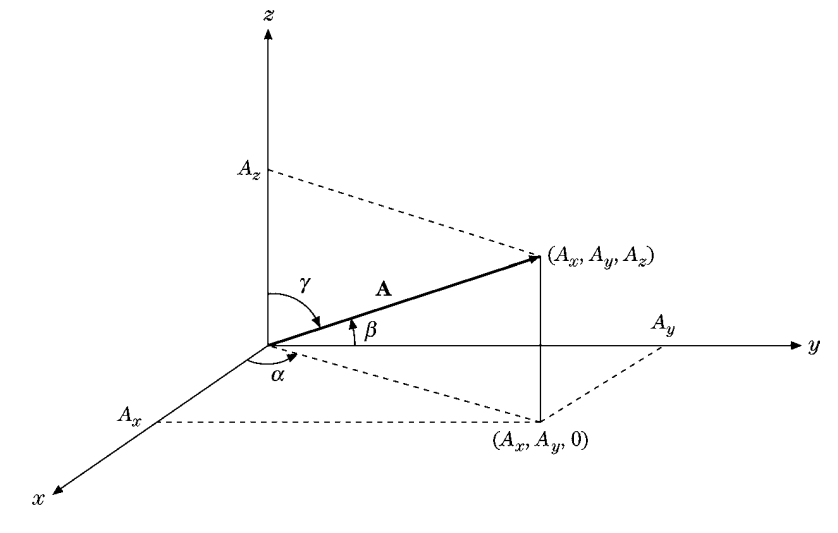
\includegraphics[width=0.6\linewidth]{img/cosines.png}
        \caption{Vector components and direction cosines of A.}
        \label{fig:enter-label}
\end{figure}


    

\section{Dot Products}

\begin{definition}[Dot Product]
    $$\vect{A} \cdot \vect{B} := \sum_{i=1}^n{a_i b_i} = |\vect{A}||\vect{B}|\cos(\theta)  $$    
\end{definition}

Here are some useful properties of dot products summarized:

\begin{theorem}

(Dot product properties). 

\begin{enumerate}
  \item $\vect{a} \cdot \vect{a} = |\vect{a}|^2$
  \item $\vect{a} \cdot \vect{a} = 0 \iff \vect{a} = 0 $
  \item $\vect{a} \cdot \vect{b} = \vect{b} \cdot \vect{a} $ (Commutativity) 
  \item $\vect{a} \cdot (\vect{b} + \vect{c}) = (\vect{a} \cdot \vect{b}) + (\vect{a} \cdot \vect{c})$ (Distributivity Over Addition)
  \item $(k\vect{a}) \cdot \vect{b} = \vect{a} \cdot (k\vect{b}) $ (Scalar Associativity)
  
\end{enumerate}
    
\end{theorem}
We can use the dot product to more compactly define the projection of one vector onto another. Consider the following scenario: 


\begin{figure}[H]
    \centering
    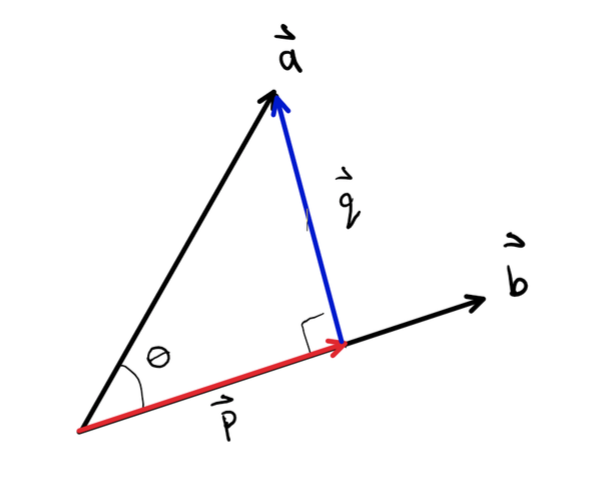
\includegraphics[width=0.5\linewidth]{img/proj.png}
    \caption{Vector Projection}
\end{figure}

We want to describe the vector $\vect{p}$, which is the projection of $\vect{a}$ onto $\vect{b}$, in terms of the dot product. Clearly, $|\vect{p}| = |\vect{a}|cos(\theta)$. We also know the direction of $\vect{p}$, which is the same as the direction of $\vect{p}$, or $\frac{\vect{b}}{|\vect{b}|} $. Thus, we have 

\begin{align*}
    \vect{p} &= |\vect{a}|\cos(\theta) \frac{\vect{b}}{|\vect{b}|} \\
             &= |\vect{a}|\frac{|\vect{b}|}{|\vect{b}|} \cos(\theta)  \frac{\vect{b}}{|\vect{b}|} \\
             &= \frac{\vect{a} \cdot \vect{b}}{|\vect{b}|} \uvect{b}
\end{align*}


\begin{definition}
    The \textbf{projection} of $\vect{a}$ onto $\vect{b}$, or $\textbf{proj}_b(a)$, is defined as 

   $$ \textbf{proj}_b(a) = |\vect{a}\cos(\theta)|\uvect{b} = \frac{\vect{a} \cdot \vect{b}}{|\vect{b}|} \uvect{b} 
   = \frac{\vect{a} \cdot \vect{b}}{\vect{b} \cdot \vect{b}} \uvect{b}  $$
\end{definition}

\section{Cross Products}
\begin{definition}
    The \textbf{cross product} of two vectors is 
    \begin{displaymath}
        \vect{a} \cross \vect{b} = 
        \begin{vmatrix}
            \ihat & \jhat & \khat \\
            a_i & a_j & a_k \\
            b_i & b_j & b_k \\
            
        \end{vmatrix}
    \end{displaymath}
    Where the direction of the resulting vector follows the right-hand rule. Additionally, the magnitude of the cross product is
 \begin{displaymath}
    |\vect{a} \cross \vect{b}| = |\vect{a}||\vect{b}|\sin(\theta)
 \end{displaymath}

    
\end{definition}

 Some useful properties of cross products are summarized below: 

 \begin{theorem}
  (Cross Product Properties). \    
    
\begin{enumerate}
  \item $\vect{a} \cross \vect{a} = 0$ 
  \item $\vect{a} \cross \vect{b} = - \vect{b} \cross \vect{a} $ (Anticommutativity) 
  \item $\vect{a} \cross (\vect{b} + \vect{c}) = (\vect{a} \cross \vect{b}) + (\vect{a} \cross \vect{c})$ (Distributivity Over Addition)
  \item $(k\vect{a}) \cross \vect{b} = \vect{a} \cross (k\vect{b}) $ (Scalar Associativity)
  
\end{enumerate}
 \end{theorem}
 


Finally, we summarize some useful vector derivative formulas below.

\begin{definition}

    (Vector Derivative Identities). Let $\vect{A}$, $\vect{B}$, be time-varying vectors and let
    $a(t)$ be a scalar-valued function of time. Then \
   \begin{itemize}
    \centering
    \item $\dv{t}(a(t)\vect{A}) = \vect{A} \dv{a}{t} + a(t)\dv{\vect{A}}{t}$
     
    \item $\dv{t}(\vect{A} \cdot \vect{B}) = \vect{A} \dv{\vect{B}}{t} + \vect{B}\dv{\vect{A}}{t}$

    \item $\dv{t}(\vect{A} \cross \vect{B}) = \dv{\vect{A}}{t}\cross\vect{B} +  \vect{A} \cross \dv{\vect{B}}{t}$
   \end{itemize} 
    
\end{definition}


\section{Taylor Series and Differentials}

Suppose we have a function that we want to express as a power series: 

\[
f(x) = a_0 + a_1 x + a_2 x^2 + a_3 x^3 + \dots
    \]

To find the coefficients of this expression, we can first observe that

\[ 
    a_0 = f(0)
\]

To find the next coefficients, we can differentiate: 

\begin{align*}
    a_1 &= f'(0) \\
    a_2 &= \frac{f''(0)}{2!} \\
    a_3 &= \frac{f'''(0)}{3!} \\
        &\dots \\
\end{align*}

Thus, combining our results we have 

\[
    f(x) = f(0) + f'(0)x + \frac{1}{2}f''(0)x^2 + \frac{1}{3!}f'''(0)x^3 + \dots 
\]

In general, the Taylor Series centered at an arbitrary input value $a$ is 

\begin{definition}[Taylor Series]
    \label{def:tseries}
    \[
        f(a+x) = f(a) + f'(a)(x) + \frac{1}{2}f''(a)x^2 + \frac{1}{3!}f'''(a)x^3 + \dots 
        \]
    
\end{definition}

The following is a list of common Taylor expansions: 

\begin{theorem}
(Common Taylor Expansions). \
\begin{enumerate}
    \item $\sin(x) = x - \frac{1}{3!}x^3 + \frac{1}{5!}x^5 + \dots \approx x $ (for small $x$)
    \item $\cos(x) = 1 - \frac{1}{2}x^2 + \frac{1}{4!}x^4 + \dots \approx 1 - \frac{1}{2}x^2 $ (for small $x$)
    \item $e^{x} = 1 + x + \frac{1}{2!}x^2 + \frac{1}{3!}x^3 + \dots $ (Valid for all $x$) 
    \item $\frac{1}{1 \pm x} = 1 \mp x + x^2 \mp x^3 + \dots$ (Only valid for $-1 < x < 1$)
    \item $\frac{1}{\sqrt{1 + x}} = 1 - \frac{1}{2}x + \frac{1}{8}x^2 + \dots$ (Only valid for $-1 < x < 1$)
    \item $(1+x)^n = 1 + nx + \frac{n(n-1)}{2!} x^2 + \frac{n(n-1)(n-2)}{3!} x^3 + \dots$ (Only valid for $-1 < x < 1$) 
    

\end{enumerate}    
\end{theorem}

Using the Taylor series, we can now construct a useful approximation for differentials. 
Consider the Taylor series of $f(x+\Delta x)$. By Definition \ref{def:tseries}, 

\[
    f(x+\Delta x) = f(x) + f'(x)\Delta x + \dots
\]

Discarding higher-order terms, we note that 

\[
    \frac{\Delta f}{\Delta x} \approx f'(x)
\]

\end{document}

